\documentclass[a4paper,12pt]{article}
\usepackage[spanish]{babel}
\usepackage{graphicx}
\usepackage{geometry}

\begin{document}

\newgeometry{top=10cm,bottom=2cm,left=3cm,right=3cm}
\begin{titlepage}
\begin{center}
{\Huge Informe de proyecto Moogle!}\\
\vspace{0.5cm}
{\Large Jean Carlo García Wong}
{\large Julio,2023}
\begin{figure}[h]
    \center{}
    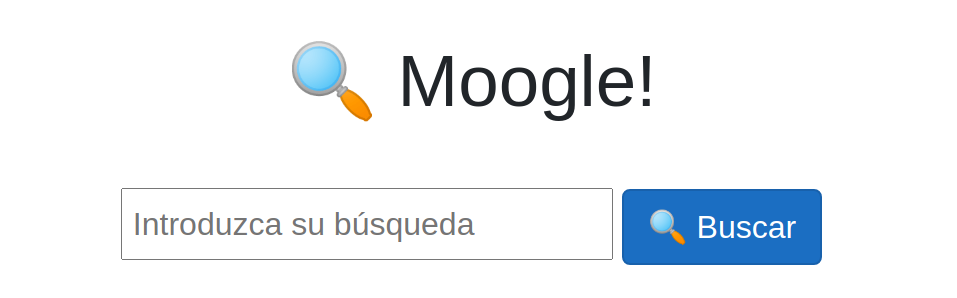
\includegraphics[width=12cm]{moogle.png}
\end{figure}
\end{center}
\end{titlepage}
\restoregeometry

\newpage
\begin{abstract}
    Moogle! 
    es un buscador de texto en el cual el usuario puede realizar
    una búsqueda inteligente entre varios textos de contenidos
    diversos ya sea con fines investigativos o solo por curiosidad 
    de una manera sencilla y eficaz.
\end{abstract}

\section{Introducción}\label{sec:intro}
    En este proyecto de programación hemos usado varios algoritmos
    que son reconocidos mundialmente como los mejores para estas 
    cuestiones de búsqueda de textos, entre los cuales se encuentran
    el TF*IDF el cual me permite determinar que tan parecidos son dos textos sin importar su longitud.

    Moogle! es de una gran importancia para mi desarrollo como programador
    porque con él he podido ver cuales son los buenos habitos que todo coder
    debe tener a la hora de realizar sus proyectos, me ha servido como otra
    materia de estudio donde he aprendido mucho sobre los algoritmos mencionados
    anteriormente y ha aumentado el amor hacia mi carrera Ciencias de la Computación.
    
    \newpage
    \section{Ejecución}
    Al ejecutar mi programa el usuario debe ingresar su búsqueda entonces desde
    ahí cargo todos los archivos de texto y posterior a esto analizo la consulta
    que ingresó el usuario para saber si empleó algunos de los operadores de búsqueda
    que estan implementados en este proyecto y eliminar además elementos que no presenten
    relevancia, todo lo anterior se realiza para determinar de que manera se debe operar
    con los documentos.
    \subsection{Análisis de la consulta}
    Para analizar lo que el usuario quiere que sea encontrado hago uso de una función 
    llamada SplitList la cual uso para fragmentar la consulta haciendo un mejor análisis
    de esta.
    \subsection{Evaluación de la búsqueda}
    Después de haber parseado la consulta hago uso de un método llamado ComputeScore el cual
    se encarga de darle valor a los documentos en dependencia de que tan parecidos sean a lo que
    el usuario desea encontrar, esto se realiza con el algoritmo TF*IDF y en él influyen los 
    operadores de búsqueda. Luego hago uso del método llamado numeroDocs que me da
    previamente en cuantos documentos se encuentra cada palabra de la consulta ingresada por el usuario,
    después se analiza si el usuario empleo algún operador en la consulta, en caso cierto se realiza 
    la funcionalidad del operador. Posteriormente se calcula el valor del TF*IDF que ya habiamos mencionado
    anteriormente:

    \begin{equation}\label{eq:grav}
        TF = \frac{x}{T}       idf  = \log {\frac{N}{n}}
    \end{equation}
    \begin{equation}
        idf  = \log {\frac{N}{n}}
    \end{equation}
    \begin{equation}
        TF\ast idf
    \end{equation}

    \begin{itemize}
        \item TF\@: Term Frequency.
        \begin{itemize}
            \item x\@: Cantidad de veces que aparece el término.
            \item T\@: Cantidad total de palabras del vocabulario de todos los documentos.
        \end{itemize}
        \item idf: Inverse Document Frequency.
        \begin{itemize}
            \item N\@: Cantidad total de documentos.
            \item n\@: Cantidad de documentos en los cuales se encuentra la consulta.
        \end{itemize}
    \end{itemize}

    Para terminar la evaluación de los documentos se hace uso del método ComputeSnippet el cual nos otorga 
    una cadena de texto de una longitud aproximada de 50 palabras en la que se puede apreciar
    el resultado de la búsqueda.
    
    Pero. ¿Qué pasaría si el usuario por alguna razón se equivoca escribiendo su consulta?
    Bueno para esta interrogante existe el algoritmo llamado Damareau-Levenshtein el cual describo en breve a continuación.

    \subsection{Damareau-Levenshtein}
        Damareau-Levenshtein a modo resumen es un método que se encarga de ver que si no se encontro nada
        relacionado con lo que el usuario escribió exactamente y en caso positivo busca una posible consulta
        lo más parecida a lo que el usuario quizo decir y luego sigue el hilo de la ejecución explicado anteriormente.

    \section{Almacenamiento de información}
        Luego de haber calculado el score de cada documento almacenaremos 
        la información de los resultados de la búsqueda en cada documento,
        para esto implementé una clase nueva llamada DocsFinal de la cual hablaré
        más tarde, esto se hace con el método doRanking el cual separa en una lista
        de DocsFinal aquellos documentos que tengan un score mayor que 0.

        Esto no se hubiera logrado sin la clase DocsFinal la cual me permite almacenar
        el nombre del documento, su snippet y su respectivo score para luego hacer 
        un ordenamiento de todos los documentos según su valor de score, recalcar que 
        los documentos se ordenan de mayor score a menor. Dentro de esta clase use los métodos
        CompareTo y Equals los cuales los implementan las interfaces IEquatable y IComparable.
        Por último se crean los SearchItem y los SearchResult con los documentos ya listos para
        posteriormente mostrárselos al usuario retornándolos en el método principal Query.
        
        \newpage
        \section{Concluciones}
        Este proyecto me ha sido de gran utilidad como aprendizaje, me ayudó a mejorar mi enfoque de programación
        y a saber la realidad de como es el día a día de un coder. Además aprendí un montón de malos hábitos que
        deben ser evadidos por cualquier persona que tenga conocimiento de la programación. Espero que haya sido de utilidad este informe.

        \newpage
        \section{Recomendaciones}
            En este proyecto vi mas conveniente representar los documentos en diccionarios por la facilidad
            que me dan a la hora de trabajar por su par Key-Value el cual me da una gran facilidad para operar sobre
            los documentos y sus respectivos valores de score y además me facilita el trabajo sobre la clase DocsFinal
            para almacenar todos los documentos ordenados por su score.
        
        \newpage
        \tableofcontents
        
    \end{document}
    